\documentclass[preprint,11pt]{elsarticle}
\usepackage[style=numeric, sorting=none, backend=biber]{biblatex}

%% Use the option review to obtain double line spacing
%% \documentclass[preprint,review,12pt]{elsarticle}

%% Use the options 1p,twocolumn; 3p; 3p,twocolumn; 5p; or 5p,twocolumn
%% for a journal layout:
%% \documentclass[final,1p,times]{elsarticle}
%% \documentclass[final,1p,times,twocolumn]{elsarticle}
%% \documentclass[final,3p,times]{elsarticle}
%% \documentclass[final,3p,times,twocolumn]{elsarticle}
%% \documentclass[final,5p,times]{elsarticle}
%% \documentclass[final,5p,times,twocolumn]{elsarticle}

%% The graphicx package provides the includegraphics command.
%\usepackage{graphicx}
%% The amssymb package provides various useful mathematical symbols
\usepackage{amssymb}
%% The amsthm package provides extended theorem environments
%% \usepackage{amsthm}

%% The lineno packages adds line numbers. Start line numbering with
%% \begin{linenumbers}, end it with \end{linenumbers}. Or switch it on
%% for the whole article with \linenumbers after \end{frontmatter}.
\usepackage{lineno}

%% natbib.sty is loaded by default. However, natbib options can be
%% provided with \biboptions{...} command. Following options are
%% valid:

%%   round  -  round parentheses are used (default)
%%   square -  square brackets are used   [option]
%%   curly  -  curly braces are used      {option}
%%   angle  -  angle brackets are used    <option>
%%   semicolon  -  multiple citations separated by semi-colon
%%   colon  - same as semicolon, an earlier confusion
%%   comma  -  separated by comma
%%   numbers-  selects numerical citations
%%   super  -  numerical citations as superscripts
%%   sort   -  sorts multiple citations according to order in ref. list
%%   sort&compress   -  like sort, but also compresses numerical citations
%%   compress - compresses without sorting
%%
%% \biboptions{comma,round}

% \biboptions{

%   --------------------------------------------------------------------
%       Text dimensions
%   --------------------------------------------------------------------
\usepackage[dvips]{geometry}
\geometry{letterpaper,left=3.0cm,right=2.0cm,top=3.0cm,bottom=2.0cm}

\usepackage[backend=biber]{biblatex}



\usepackage{adjustbox}
\usepackage{graphicx}
\usepackage{subfigure}
\usepackage[cmex10,fleqn]{amsmath}
\usepackage{nccmath}
\usepackage{algorithmic}
\usepackage{array}
%\usepackage[colorlinks=true,citecolor=blue,linkcolor=blue,urlcolor=blue,plainpages=false]{hyperref}
\usepackage[bookmarks=false,pdfstartview={FitH},colorlinks=true,citecolor=black,linkcolor=black,urlcolor=black,plainpages=false]{hyperref}
\usepackage{breakurl}
\usepackage{nomencl}
\usepackage{multirow}
\usepackage{multicol}
\usepackage{stfloats}
\usepackage{mdwmath}
\usepackage{mdwtab}
\usepackage{eqparbox}
\usepackage{amsfonts}
\usepackage{amsbsy}
\usepackage[dvipsnames]{xcolor}
\usepackage{graphicx}
\usepackage{float}

\usepackage[caption=false, font=footnotesize]{subfig}

\renewcommand\thesubfigure{(\alph{subfigure})}
\usepackage{balance}
%\usepackage{flushend}
\usepackage{booktabs, tabularx, multirow, array,makecell}
\renewcommand\theadfont{\normalfont}
\usepackage{ragged2e}
\newcolumntype{Y}{>{\hsize=1.75\hsize}X}
\newcolumntype{Z}{>{\hsize=.875\hsize\RaggedLeft}X}
\setlength\extrarowheight{1.5pt}
\usepackage{pifont}

\usepackage[spanish]{babel} % Para soporte en español
\usepackage{graphicx} % Para manejar imágenes
\usepackage[spanish]{caption} % Asegúrate de cargar caption con la opción español
\newcommand{\Blue}[1]{\textcolor{blue}{#1}}
\newcommand{\Red}[1]{\textcolor{red}{#1}}
\newcommand{\G}[1]{\textcolor{green}{#1}}
\usepackage[style=numeric, backend=biber]{biblatex}
\addbibresource{referencias.bib}


\begin{document}

\begin{frontmatter}

\title{Optimización dinámica del despacho de buses: un enfoque adaptativo a la demanda y condiciones operativas de Montería}


%% Group authors per affiliation:
\author[label1]{Martin Del Gordo}
\address[label1]{Departamento de Ingenier\'ia Industrial, Universidad de Los Andes, Colombia}
\ead{m.delgordo@uniandes.edu.co}

\author[label1]{Samuel Rubio}
\ead{s.rubioc2@uniandes.edu.co}

\author[label1]{Javier Barrera}
\ead{j.barrerahu@uniandes.edu.co}

\end{frontmatter}

\linenumbers
\section{Introducción}
\vspace{-1mm}
\label{Int}

\Blue{La eficiencia del transporte público es crucial para la calidad de vida en las ciudades y la sostenibilidad urbana. Un sistema de transporte bien gestionado minimiza los tiempos de espera, mejora la experiencia del usuario y optimiza el uso de los recursos disponibles, reduciendo la congestión vehicular, las emisiones contaminantes y el consumo de espacio urbano. Debido a esto, según el Banco Mundial\cite{worldbank_transport_2023} hoy en día uno de los principales desafios de los paises en desarrollo es garantizar que todos tengan acceso a una movilidad eficiente a partir de la modernización y optimización de las operaciones de sus sistemas de transporte público. Sin embargo, a pesar de los avances en la planificación del transporte público, muchas ciudades y regiones continúan enfrentando desafíos importantes relacionados con la elaboración de rutas, sincronización de horarios, y asignación de buses, lo que genera servicios poco confiables e ineficientes\cite{camos2020transporte}.}

\Blue{Por lo tanto, un aspecto clave en la gestión óptima del transporte público es el despacho eficiente de autobuses. Tradicionalmente, los modelos de despacho de buses se basan en horarios fijos o en reglas operativas simples, que no logran capturar adecuadamente las variaciones en la demanda de pasajeros ni las condiciones cambiantes del tráfico. Estas aproximaciones estáticas a menudo resultan en una utilización ineficiente de los recursos. En algunos casos, se observa una sobreoferta de autobuses, con vehículos subutilizados en momentos de baja demanda, mientras que en otros, la falta de buses en horarios pico provoca largos tiempos de espera y congestión de pasajeros.\cite{guihaire2008} Este desequilibrio resalta la necesidad de desarrollar modelos de despacho más sofisticados y flexibles que se adapten a las condiciones operativas, como los retrasos, el tráfico, la capacidad y cantidad de buses, y la demanda.}

En años recientes, el campo de la optimización del despacho de buses ha progresado significativamente gracias a la integración de técnicas avanzadas de modelado matemático y algoritmos de optimización. Entre las metodologías más destacadas se encuentran la programación lineal y entera, así como algoritmos heurísticos y metaheurísticos, tales como los algoritmos genéticos y la optimización por enjambre de partículas. Estos modelos avanzados permiten equilibrar múltiples objetivos, como la minimización de los tiempos de espera de los pasajeros, la reducción de costos operativos, la disminución de las emisiones contaminantes y la mejora de la confiabilidad del servicio.\cite{cheng2024bus} Sin embargo, aunque estos enfoques han demostrado ser efectivos en diversas aplicaciones, su implementación en entornos reales aún enfrenta desafíos debido a la complejidad de las operaciones y la necesidad de considerar factores impredecibles, como el tráfico y la demanda variable \cite{fakhravar2022heuristics}.

El problema de optimización del despacho de buses puede abordarse desde dos perspectivas clave: la de los usuarios y la de las empresas operadoras. Por un lado, las empresas buscan minimizar costos, maximizar sus utilidades y mantener una alta frecuencia de buses, lo que a menudo lleva a priorizar la eficiencia operativa sobre las necesidades de los usuarios. Por otro lado, los usuarios demandan un servicio de transporte cómodo, accesible, puntual y eficiente. Estas diferencias en las prioridades crean una tensión natural entre los objetivos empresariales y las expectativas de los pasajeros, lo que hace que encontrar una solución que equilibre ambos intereses sea complejo. Diversos autores plantean soluciones basadas en sus respectivos enfoques, tal como se evidencia en \cite{guihaire2008}. Actualmente, el desafío consiste en desarrollar un sistema que logre una asignación óptima de recursos, capaz de satisfacer la demanda de los usuarios, mejorar su experiencia de transporte y, al mismo tiempo, optimizar las operaciones para las empresas.

\Blue{Dado los problemas identificados en el sistema de transporte público, este documento se enfoca en la ciudad de Montería, Colombia, la cual enfrenta importantes desafíos de movilidad que han impactado negativamente a los usuarios, las empresas de transporte y el comercio local. Según Fenalco, la situación en Montería es especialmente preocupante debido a una crisis financiera y operativa que viene afectando desde hace algunos años a las empresas del sector.\cite{fenalco2024transporte}. Las empresas de transporte no han podido ofrecer un servicio eficiente, lo que les ha generado grandes perdidas y las ha obligado a reducir tanto las rutas como la frecuencia de los buses ofrecidas en sus ofertas, causando un incremento significativo en los tiempos de espera y disminuyendo la calidad del servicio, razones que junto al crecimiento del transporte informal e ilegal se señalan como las principales causas de la desincentivación de las personas a movilizarse por este medio. \cite{ortiz2023transporte}.}

\Blue{Este panorama en Montería refleja problemas estructurales y logísticos similares a los experimentados en otras ciudades de Colombia. Tal como señalan Gibet Camós y Juanita Concha, la implementación de sistemas de transporte masivo, como el MIO en Cali, ha dejado importantes lecciones sobre la consolidación de estos sistemas. La calidad deficiente del servicio, la frecuencia inadecuada y el aumento del transporte informal, junto con la dependencia de los ingresos por tarifas, han impedido la efectividad de estos sistemas \cite{camos2020transporte}. En Montería, las empresas de transporte han experimentado pérdidas significativas, y la mejora del servicio se plantea como una solución necesaria para revertir esta situación \cite{fenalco2023perdidas}. 
Por lo tanto, ante la clara necesidad de los operadores del transporte urbano de soluciones cada vez mas soficisticadas para realizar la planificación de la operación de sus flotas, este trabajo pretende atacar esta problematica mediante el desarrollo de un modelo de flujo en redes que permita optimizar la programación y despacho de buses en el sistema de transporte público de Montería. Además, se busca que la toma de decisiones del modelo sea dinamica basandose en factores como la variabilidad en los flujos de usuarios, la capacidad de los vehículos y los tiempos de tránsito. Finalmente se evalua el desempeño del modelo propuesto evaluando que efectivamente este halla incrementado el nivel de servicio de los usuarios y generado una utilización eficiente de los buses.}
 
\section{Estado del Arte}
\vspace{-1mm}
\label{Int}

\subsection{Clasificación de problemas asociados con la planificación de transporte público}

Usualmente, los problemas de medios de transporte público se dividen en cinco diferentes tipos de objetivos. El primer tipo de problema es el diseño de rutas, este se centra en planificar y definir las distintas rutas de transporte público con el objetivo de satisfacer las necesidades de los usuarios y al mismo tiempo las de la empresa. Segundo, la frecuencia de los buses para generar satisfacción en los clientes. Tercero el horario de cada ruta y la salida de los buses para mantener un sistema estable en el medio de transporte. Cuarto, la programación de los distintos tipos de vehículos en el sistema, y, por último, la programación de los empleados, quienes son responsables de que el sistema funcione. Cada uno de estos objetivos cuenta con distintos supuestos necesarios para llegar a una solución, lo que contribuye a que el sistema de transporte público sea multiobjetivo, dificultando el análisis y las diversas soluciones. \Blue{\cite{guihaire2008}}

Estos problemas son de gran complejidad y, cada año, con el avance de la tecnología, se obtienen respuestas más rápidas y mejores. Sin embargo, la solución de un sistema de transporte, aunque se aborde desde distintas perspectivas, sigue siendo considerada un problema NP-Hard \cite{magnanti1984}. Un problema NP-Hard, o problema NP-duro, es aquel cuya complejidad es tal que no se puede reducir el tiempo de obtención de resultados. Estos problemas son tan difíciles de resolver que no existen algoritmos que puedan resolverlos en tiempo polinómico.

El primer tipo de problema abordado en la planificación del transporte público es el diseño de rutas o \textit{Transit Network Design Problem} (TNDP). El objetivo principal de este problema es determinar las rutas óptimas por las cuales los autobuses deben operar, incluyendo la ubicación de las paradas. La solución generalmente se basa en el uso de matrices origen-destino, buscando satisfacer la demanda de la mayor cantidad posible de pasajeros. \Blue{El primer enfoque sobre este problema fue presentado por Patz en 1925 \parencite{patz1925}, quien planteó un modelo con el objetivo de minimizar el número de asientos vacíos en los autobuses, considerando la capacidad del vehículo y la demanda en cada sitio. A lo largo del tiempo, varios autores han propuesto diferentes restricciones para mejorar la solución del TNDP.} Por ejemplo, Murray \parencite{murray2003} sugiere la consideración de características como la cobertura de las rutas, la longitud de estas, la densidad de pasajeros y las ubicaciones de las paradas. En otro estudio, Murray \parencite{murray1998} introduce la condición de que el nivel de satisfacción de la demanda debe ser superior al 90\%, teniendo en cuenta las distintas longitudes de las rutas y los tipos de autobuses. \Blue{Estos estudios destacan la importancia de factores como la longitud de las rutas, la densidad de pasajeros, el número de paradas y la demanda, como elementos clave para la solución del TNDP.}

\Blue{El segundo tipo de problema, conocido como establecimiento de frecuencias o \textit{Transit Network Frequency Setting Problem} (TNFSP), se enfoca en determinar la frecuencia con la que los autobuses deben operar en rutas predefinidas para satisfacer la demanda de pasajeros. Scheele \parencite{scheele1980} fue uno de los primeros en abordar este problema, proponiendo un modelo cuyo objetivo es minimizar el tiempo que los pasajeros pasan a bordo de los autobuses, mientras se considera la capacidad de los vehículos y la disponibilidad de la flota. Por su parte, Furth \parencite{furth1982} se enfoca en maximizar el número de pasajeros transportados y minimizar el tiempo de espera en las paradas, teniendo en cuenta las restricciones impuestas por el tamaño de la flota y el presupuesto disponible. Evidenciando dos formas diferentes en aboradar el problema.}

El tercer tipo de problema es el de asignación de horarios o \textit{Transit Network Timetabling Problem} (TNTP). Este problema busca \Blue{establecer los horarios óptimos de salida de los autobuses desde las terminales}, el tiempo total para completar una ruta y las horas estimadas de llegada a cada parada. \Blue{Guihaire \parencite{guihaire2008} señala que los elementos clave en la solución de este problema incluyen la satisfacción de la demanda, la coordinación de las transferencias entre rutas, el tamaño de la flota y la reutilización de horarios previamente establecidos. Chakroborty \parencite{chakroborty1995} presentó uno de los primeros enfoques al respecto, con el objetivo de minimizar el tiempo total de espera de los pasajeros, utilizando restricciones como el tamaño de la flota, la capacidad de los vehículos y el número máximo de transferencias. Otro enfoque relevante fue propuesto por Castelli \parencite{castelli2004}, quien se centra en minimizar el tiempo de transferencia, considerando las frecuencias y rutas previamente establecidas.}

\Blue{El cuarto tipo de problema es el problema de diseño de rutas y establecimiento de frecuencias o \textit{Transit Network Design and Frequency Setting Problem} (TNDFSP), que combina los enfoques de los problemas TNDP y TNFSP. Este problema tiene como objetivo simultáneo diseñar las rutas óptimas y determinar la frecuencia de los autobuses en esas rutas. Uno de los primeros modelos fue desarrollado por Lampkin en 1967 \parencite{lampkin1967}, quien se enfocó en maximizar el número de pasajeros transportados directamente y minimizar su tiempo total de viaje, bajo la restricción de la capacidad de los autobuses. En un estudio más reciente, Borndorfer \parencite{borndorfer2005} abordó el problema en la ciudad de Postdam, con el objetivo de minimizar el tiempo de viaje de los pasajeros y los costos operativos, respetando la demanda del sistema de transporte.}

\Blue{El último tipo de problema es el problema de asignación de frecuencias y horarios o \textit{Transit Network Scheduling Problem} (TNSP), que combina los enfoques del TNFSP y el TNTP. Este problema tiene como objetivo determinar las frecuencias de los autobuses y, con base en estas, generar los horarios de salida y llegada en las paradas. Eranki \parencite{eranki2004} aborda este problema buscando minimizar el tiempo de espera de los pasajeros, bajo la restricción de no exceder un tiempo máximo de espera y estableciendo la coordinación de llegadas simultáneas entre diferentes rutas.}


De esta forma, se evidencia la complejidad de los distintos problemas y su relación, lo que complica el entendimiento de los sistemas de transporte público. Estos problemas se pueden comprender como se muestra en {la Figura.\ref{fig:mi_imagen1}, propuesta por \cite{guihaire2008}}.

\captionsetup[figure]{name=Figura}
\begin{figure}[H]
  \centering
  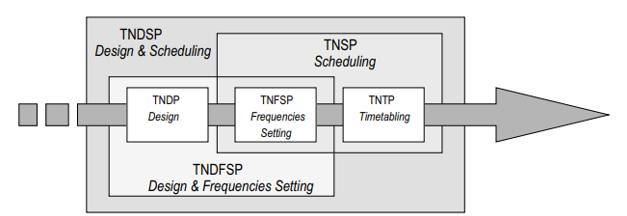
\includegraphics[width=0.8\textwidth]{tipos.png}
  \caption{Tipos de problemas en medios de transporte}
  \label{fig:mi_imagen1}
\end{figure}


Con el entendimiento de estos problemas se puede evidenciar el desarrollo y conocimiento del estado del arte. A continuación, se evidencia el estado del arte en los distintos tipos de problemas.

\subsection{Enfoques para solucionar el problema TNT}

Haciendo uso de lo mencionado anteriormente, se evidencian los distintos problemas en el planteamiento de un sistema de transporte público, así como las diferentes perspectivas, objetivos, supuestos y restricciones abordados por cada autor, lo que resulta en una amplia gama de soluciones.

Teniendo en cuenta estos problemas, se debe considerar el proyecto a trabajar, es un problema TNTP. \Blue{El problema de despacho óptimo de vehículos en Monteria} se alinea con el TNTP, ya que se busca establecer los distintos horarios de los buses de salida de la terminal para cumplir con la mayor demanda posible, generando satisfacción en los clientes y aumentando el consumo del medio de transporte, directamente relacionado con los ingresos generados por este uso. \Blue{Existen diversos enfoques para abordar este tipo de problemas. A lo largo de los años, se han propuesto varios modelos matemáticos y técnicas de optimización en la literatura académica. A continuación, se describen los enfoques más relevantes, sus características principales, y cómo pueden aplicarse a la solución del problema en Montería.}


\Blue{\subsubsection{Métodos basados en programación lineal}}

\Blue{Uno de los enfoques más utilizados para la optimización del despacho de vehículos en transporte público es la programación lineal. Este enfoque se centra en formular el problema como un conjunto de ecuaciones lineales que representan las restricciones operativas, como la capacidad de los autobuses, los horarios de operación y la demanda de pasajeros. Generalmente suele tener como objetivo minimizar los costos operativos o maximizar la eficiencia del sistema mediante.}

Por ejemplo, el artículo \cite{borndorfer2005} aborda el problema de determinar las frecuencias óptimas de autobuses con el objetivo de minimizar los costos operativos y los tiempos de viaje de los pasajeros. \Blue{Para plantear este problema, los autores emplean matrices origen-destino que modelan los patrones de desplazamiento de los pasajeros entre distintos puntos en un marco temporal. A partir de estas matrices, ajustan las frecuencias de las rutas para satisfacer la demanda de transporte.}

\Blue{Los autores proponen dos modelos multiobjetivo, que buscan minimizar una combinación del tiempo total de transporte y los costos operativos. El segundo modelo considera el sistema de transporte como un grafo unidireccional donde se analiza cada ruta de manera individual. Este modelo asume que los pasajeros eligen siempre la ruta más corta y que los autobuses operan dentro de límites de capacidad específicos. Las variables clave del modelo son: la cantidad de pasajeros, la elección de una línea específica y la frecuencia de los autobuses. A través de estas variables, se calcula tanto el costo total del sistema como el tiempo total que los pasajeros pasan en el transporte.}

Debido a la complejidad del problema, que es de tipo NP-hard, se recurre a técnicas de relajación para obtener soluciones factibles. Una técnica comúnmente empleada consiste en la activación o desactivación de restricciones para generar soluciones iniciales que puedan ser refinadas posteriormente, logrando así una solución óptima.


\Blue{Existe una gran cantidad de trabajos que abordan el problema de manera similar con ligeras diferencias, como es el caso del modelo propuesto por Borndorfer et al. \cite{borndorfer2005} el cual continua en esta línea del modelado lineal pero con un enfoque hacía la conservación de los flujos dentro del sistema, lo que garantiza la estabilidad del mismo, y la necesidad de no exceder la capacidad de los autobuses ni la demanda esperada, evitando así la sobrecarga del sistema.} 

\Blue{
Por otro lado, tambien se presentan enfoques con mas tendencia hacía la simulación como el propuesto por Wang et al. \cite{wang2017}, el cuál se enfoca en calcular el tiempo de salida y llegada de los autobuses a cada estación, así como la asignación de los pasajeros a los buses y su tiempo de espera. Curiosamente, este modelo no cuenta con la información precisa de la hora de llegada de los pasajeros a las estaciones. Para resolver esto, los autores asumen que el tiempo de espera de cada pasajero sigue una distribución de probabilidad, la cual está indexada por ruta, ya que las expectativas de arribo pueden variar según la línea de bus. Lo anterior permite transformar el modelo a uno que no busca directamente satisfacer la mayor cantidad de demanda posible a diferencia de los anteriores, sino minimizar el tiempo de espera de cada pasajero. Al reducir el tiempo de espera, también se disminuye la probabilidad de que los pasajeros abandonen la estación, lo que optimiza la demanda cumplida\cite{wang2017}. El modelo incluye una restricción de capacidad para cada autobús, considerando factores como la estación donde los pasajeros suben y bajan, lo cuál lo hace algo complejo de adaptar a sistemas como el de Monteria donde no existen paraderos u estaciones. Otra desventaja que tiene este modelo es que como parámetro se debe establecer la hora de salida del último bus. Lo anterior resulta conflictivo, pues lo ideal sería que fuera directamente el modelo el que dictaminara este tiempo. Los autores establecen que el modelo que plantean se resuelve como un MIP (Mixed-Integer Programming) usando el oprimizador CPLEX. Este optimizador utiliza algoritmos simlex para resolver problemas de optimización de tipo lineal.} 



\subsubsection{Métodos basados en programación no lineal}
\Blue{La programación no lineal es adecuada para problemas donde las relaciones entre las variables no son estrictamente lineales. Esto es común en sistemas de transporte público, donde los costos operativos y los tiempos de espera pueden depender de múltiples factores de manera no lineal.}

\Blue{En el trabajo de Dirk L. van Oudheusden y William Zhu \cite{vanoudheusden1995} se desarrolla un modelo no lineal para establecer horarios y frecuencias óptimas de autobuses, considerando las limitaciones de la flota y la capacidad de los depósitos. El objetivo del modelo es reducir los costos operativos reduciendo los viajes en vacío y aumentar el número de pasajeros transportados, incrementando así los ingresos del sistema. A su vez, el modelo busca garantizar un nivel adecuado de servicio, respetando las restricciones de capacidad de los autobuses, el tiempo máximo de espera de los pasajeros y los límites de ocupación. Para ello, los autores introducen varios supuestos clave: el tiempo de trayecto varía durante el día, la demanda de pasajeros es asimétrica y no se considera el tiempo necesario para el desplazamiento entre depósitos y las rutas.}

 \Blue{Dada la dificultad para resolver este modelo directamente, el modelo se resuelve aproximandolo a uno lineal, relajando algunas restricciones para obtener soluciones factibles. Herramientas como TURBO-Simplex 3.0 y dBASE IV 1.0 permitieron resolver estas aproximaciones, proporcionando resultados cercanos al óptimo, que fueron utilizados en el sistema de transporte de Bangkok.}

\Blue{Por su parte, en el artículo \cite{kim2009} se propone un enfoque dinámico para la optimización de las frecuencias y los horarios de autobuses en Seúl, Corea del Sur \cite{kim2009}. Los autores desarrollan un modelo no lineal que ajusta las frecuencias de los autobuses en función de la demanda fluctuante y las condiciones de tráfico en tiempo real. Entre los factores que se consideran  se incluye los costos operativos, los tiempos de viaje, la aceleración promedio y la capacidad de los autobuses. Además, se tiene en cuenta el tiempo de espera de los pasajeros, con el objetivo de minimizarlo idealmente a cero.}

\Blue{El análisis también aborda los costos asociados al tiempo que los pasajeros permanecen dentro del autobús, destacando que una mayor congestión no solo afecta la comodidad, sino que también incrementa los costos operativos y reduce la demanda del servicio. La optimización de las frecuencias permite minimizar tanto los tiempos de espera como los costos operativos. Sin embargo, los autores subrayan que la frecuencia no puede aumentarse indefinidamente, ya que está limitada por la cantidad de autobuses disponibles en la flota. Una vez que se ha determinado la frecuencia óptima, el modelo permite programar las paradas de los autobuses, considerando además otros factores como los costos de combustible y el tiempo total que los autobuses pasan en operación.}

\Blue{Este enfoque es especialmente relevante para la planificación de la demanda continua, ya que permite ajustar las variables y restricciones del sistema de transporte en función de las condiciones reales y cambiantes, ofreciendo una solución más flexible y eficiente.}

\Blue{Por otro lado, artículos como \cite{guan2023,chen2019} introducen un enfoque para optimizar la asignación de vehículos en redes de tránsito modular (MTNS). El objetivo principal es maximizar la eficiencia operativa del sistema de transporte público mediante el uso de vehículos modulares, es decir,  que pueden ajustar su capacidad en tiempo real acoplando o desacoplando módulos a lo largo de la ruta. Esto permite adaptarse mejor a la demanda de pasajeros y evita los desajustes que ocurren en sistemas tradicionales de capacidad fija, donde los vehículos pueden quedar subutilizados o sobrecargados.}

\Blue{El modelo de optimización \cite{guan2023} se formula como un problema de programación no lineal de enteros mixtos (MINLP), cuyo objetivo es minimizar los costos operativos, y con esto la distancia recorrida por los vehículos y el tiempo de espera de los pasajeros. Entre las restricciones del modelo se encuentran la capacidad de los vehículos, la conservación de los vehículos en las estaciones, y la restricción de flujo de pasajeros, que garantiza que cada pasajero complete su viaje, ya sea de forma directa o mediante transbordos. Estas restricciones son de gran relevancia ya que se pueden adaptar a las caracteristicas del sistema de Montería por lo que mas adelante seran tenidas en cuenta.}

\Blue{El principal desafío del modelo radica en su complejidad debido a la interacción de las decisiones sobre la frecuencia de los vehículos y la capacidad modular en cada enlace. Para hacer el problema más manejable computacionalmente, se reformula como un modelo de programación lineal entera mixta (MILP), lo que permite resolverlo usando herramientas como el optimizador Gurobi.}

\Blue{Los resultados de los casos de estudio en China muestran que este sistema modular reduce significativamente tanto los costos operativos como los tiempos de viaje de los pasajeros, en comparación con sistemas de capacidad fija y transporte privado. }

\Blue{Aunque el sistema que se abordara no cuenta con vehículos modulares, algunos conceptos del artículo, como la optimización de la frecuencia y la capacidad en función de la demanda, podrían ser adaptados. Ajustar la frecuencia de los autobuses según la demanda real o proyectada podría reducir costos operativos y mejorar la eficiencia del sistema, evitando despachos innecesarios y atendiendo mejor la demanda en momentos crítico.}

\Blue{Otro enfoque de modelo no lineal se desarrolla en el artículo \cite{gkiotsalitis2019}, el cual introduce un enfoque de programación robusta que optimiza los horarios de autobuses para garantizar la resiliencia del sistema ante incertidumbre en tiempos de viaje y demanda. Este modelo emplea conjuntos de incertidumbre, en lugar de distribuciones de probabilidad para modelar las llegadas y la demanda, lo que permite anticiparse a una mayor variedad de escenarios adversos sin depender de estimaciones precisas de probabilidades.}

\Blue{El problema se formula como un modelo minimax, cuyo objetivo es minimizar las peores desviaciones posibles respecto a los horarios planificados, asegurando que los tiempos de viaje no se prolonguen excesivamente y afecten la operación futura. Las restricciones del modelo incluyen tiempos mínimos de descanso para los conductores y límites en los intervalos de despacho, asegurando la viabilidad operativa.}

\Blue{Para resolver el modelo, los autores combinan un algoritmo genético con programación secuencial cuadrática, generando soluciones robustas que se validan en escenarios de peor caso.}

\Blue{Una de las grandes contribuciones de este trabajo es su capacidad para generar horarios que se desempeñan bien en escenarios de peor caso sin requerir estimaciones precisas de la probabilidad de las perturbaciones. Los autores argumentan que los horarios generados por enfoques que dependen de distribuciones de probabilidad tienden a fracasar cuando las perturbaciones reales caen fuera de las regiones de alta probabilidad de esas distribuciones, lo que motiva el enfoque robusto basado en incertidumbre presentado en este articulo.}


\subsubsection{Algorítmos de despacho dinamico}
Uno de los enfoques más innovadores para la optimización del despacho de buses es el uso de algoritmos dinámicos, que ajustan los despachos en tiempo real en función de las fluctuaciones en la demanda de pasajeros y las condiciones del tráfico. Este tipo de modelos permite una mayor flexibilidad y capacidad de respuesta ante imprevistos operativos.


\Blue{En el artículo \cite{guan2022} se presenta un modelo capaz de adaptarse a las condiciones cambiantes del tráfico y la demanda en diferentes franjas horarias. Este modelo se estructura en dos fases: una estática y una dinámica. La primera fase utiliza un algoritmo genérico de despacho estático para establecer una base inicial la cual los autores aplican un algoritmo basado en estrategia LNS para resolverlo. LNS (por sus siglas en inglés Large Neighbourhood Search) tiene como propósito minimizar la distacia total; es decir, se busca relacionar los componentes que estén más cercanos los unos de los otros y dejar más de lado aquellos lejanos.} 
\

\Blue{La fase dinámica, se ejecuta continuamente durante la operación, utiliza un algoritmo de planificación precisa que actualiza constantemente la ruta inicial. En cuanto a la segunda fase, se propone un modelo dinámico que se esté ejecutando contínuamente a lo largo de la operación. Para esta se usa un algoritmo de planeación preciso que se aplica sobre la ruta inicial y continuamente la actualiza. El objetivo principal es minimizar el intervalo entre la hora planteada inicialmente (primera fase) y aquella que dictamine el algoritmo dinámico (segunda fase).}

\Blue{La investigación aplica una integración de dos fases que mejora y facilita la implementación de un sistema de despachos dinámico. Es de especial interés este dinamismo, ya que brinda flexibilidad a la hora de responder frente a imprevistos. También permite detectar anomalías en los servicios, lo que a su vez facilita la tarea de reducirlas o, en caso de ser posible, eliminarlas.}

\Blue{En \parencite{gkiotsalitis2020} también se plantea un modelo de despacho dinámico. Para este, se hace una planeación de la hora de salida de los buses restantes justo antes del despacho de cada bus. Inicialmente, se programa la secuencia de despachos, pero, antes de que parta el segundo autobús, el modelo se actualiza tomando como referencia la salida del primero. Esta iteración se repite entonces para cada bus con el que se cuenta en cada ruta. La función objetivo del modelo es minimizar  el cuadrado de la diferencia entre el momento en el que será programado un viaje y su valor originalmente establecido.}

Para solucionar el problema, el autor hace uso de aproximaciones del gradiente para aproximar la solución de despachos. Esta solución es considerablemente más rápida que las optimizaciones exactas calculadas con programación cuadrática. Entonces, si bien la solución que se presenta en dicho modelo no es exacta, la brecha es lo suficientemente despreciable en escenarios realistas de operación de autobuses.

\Blue{De este modelo hay cosas por remarcar que resultan de especial utilidad para este tipo de trabajos. La primera y más importante es el cómo trabaja iterativamente al momento de cada despacho para recalcular y comparar las horas de salida programada para las rutas posteriores. Al momento de programar la salida de buses, existen variables imposibles de predecir con exactitud (como el tráfico) que, si bien no se contempla directamente en este modelo, su solución permite reaccionar a pequeñas variaciones en este para garantizar una operación óptima de la flota de buses.}

Por otro lado, el artículo \parencite{zhou2023} presenta un enfoque para optimizar el despacho de autobuses en sistemas de transporte público bajo demanda utilizando un modelo de optimización en tiempo real basado en reservas, con el objetivo de minimizar el costo operativo total. Este trabajo se apoya en investigaciones previas de sistemas de transporte bajo demanda, destacando el trabajo \cite{daganzo1984} donde se introdujo el concepto de rutas flexibles ajustadas a la demanda, y en \cite{gorev2020} donde se demostró la viabilidad de estos sistemas en áreas de baja densidad de pasajeros.

El modelo plantea la asignación eficiente de vehículos de diferentes capacidades a las demandas de transporte generadas en tiempo real a través de reservas. Utiliza un modelo de correspondencia óptima basado en un grafo bipartito ponderado, donde los nodos representan vehículos y demandas, y las aristas ponderadas reflejan los costos asociados a cada asignación, considerando el desplazamiento de vehículos vacíos y las restricciones de capacidad.

Para resolver el problema, los autores emplean el algoritmo de Kuhn-Munkres, que optimiza la asignación de vehículos minimizando el costo operativo total. En comparación con un enfoque heurístico, este algoritmo ofrece una solución globalmente óptima, reduciendo significativamente los costos operativos de 195.34 CNY a 177.67 CNY por viaje. 

Este tipo de modelos es útil para sistemas bajo demanda donde se busca mejorar la eficiencia operativa y reducir costos, y su uso de grafos bipartitos puede ser adaptado para optimizar la asignación de autobuses en función de la demanda.

\section{Planteamiento del Problema}

\Blue{Actualmente, Montería cuenta con 21 rutas de transporte público, operadas por varias empresas: Metrosinu; Monteria Express, Sinumovil; Monteriana Movil. Cada ruta tiene dos cabeceras, que sirven como puntos de partida para los recorridos en ambos sentidos. El recorrido de una cabecera a la otra se conoce como un sentido de la ruta, por lo que debe ser claro que todas las rutas presentan dos sentidos, no necesariamente paralelos, por lo que su comportamiento en cuanto a demanda y tiempos de recorrido serán independientes y únicos para cada sentido a pesar de ser la misma ruta. }

\Blue{La empresa cuenta con un único tipo de bus con capacidad de 52 pasajeros. Los buses pueden ser asignados desde cualquiera de las dos cabeceras, y cada sentido de la ruta está compuesto por tramos o arcos que marcan el recorrido entre puntos clave de la ciudad. Sin embargo, estos arcos son utilizados únicamente de forma interna por las empresas como guía, ya que el sistema no cuenta con paraderos fijos ni información detallada sobre características o registros específicos en estos subtramos, lo que limita la precisión en la planificación operativa, obligando a trabajar directamente desde los sentidos de cada ruta. Cabe aclarar que los buses no inician su operación desde las cabeceras, sino que todos al salir de operación son guardados en un patio común, desde donde son despachados al momento que se requieran en las cabeceras para iniciar sus recorridos, lo que claramente implica un tiempo de transito de patio a cabecera al iniciar o reanudar la operación, y de cabecera a patio al finalizarla.}

\Blue{A cada empresa operadora se le asigna mensualmente una cantidad máxima de vehículos para operar en las rutas, teniendo en cuenta ambos sentidos. Esto significa que no todas las rutas pueden ser cubiertas de manera simultánea, y que existe un límite en la cantidad de buses que pueden circular en cada ruta. Esta restricción obliga a las empresas a gestionar de forma óptima los vehículos disponibles para satisfacer la mayor demanda posible a lo largo del día. El problema principal radica en que la programación actual del despacho de buses se basa en un método manual y rudimentario, que, aunque permite mantener la operación funcional, no optimiza la distribución de los recursos para establecer una oferta sustentada dada las caracteristicas del sistema(demanda, eventualidades, cantidad y capacidad de buses, etc) que busque maximizar la atención a los pasajeros. El proceso que lleva la empresa actualmente para programar los despachos se basa en las siguientes dos tareas.}

\begin{enumerate}
    \item \textbf{Distribución inicial de buses:} Los buses se asignan equitativamente entre los dos sentidos de cada ruta, salvo que los tiempos de tránsito entre cabeceras difieran significativamente, en cuyo caso se ajusta la proporción de buses en cada sentido. La cantidad de buses utilizados en cada hora la define el operador con base en su experiencia, asegurandose de estar dentro de los limites de vehículos permitidos para la ruta.
    \item \textbf{Cálculo de intervalos de despacho:} A partir del tiempo de tránsito promedio entre cabeceras, se calcula un intervalo de despacho para cada hora de operación (de 5:00 a.m. a 9:00 p.m.). Este intervalo se determina dividiendo el tiempo de tránsito por el número de buses disponibles, lo que establece la frecuencia de despacho desde cada cabecera.
\end{enumerate}

La operación actual le ha permitido a la empresa alcanzar un IPK promedio de 0.7 pasajeros por kilómetro por ruta. Si bien este enfoque básico permite una operación inicial con cierta regularidad, los intervalos de despacho se desajustan una vez los buses comienzan a circular. Esto ocurre debido a la variabilidad en los tiempos de retorno de los vehículos, que dependen de factores como el tráfico y las condiciones específicas de la ruta. Los buses solo están disponibles para ser despachados una vez completan su recorrido, lo que provoca desfases respecto al intervalo planificado inicialmente.

Además de estos problemas operativos, el método de despacho actual no considera un factor clave: la demanda de pasajeros. La cantidad de usuarios varía significativamente según la hora del día, el día de la semana, e incluso factores estacionales o eventos imprevistos que son cotidianos en este tipo de actividad. Al no tomar en cuenta estos factores, el sistema actual puede asignar demasiada capacidad en momentos de baja demanda, o insuficiente capacidad en las horas pico. \Blue{Esto genera tiempos de espera prolongados y una utilización ineficaz de los recursos, lo que afecta tanto la experiencia de los usuarios como los costos operativos de las empresas.}

No obstante, también se presentan importantes limitaciones con los datos históricos que la infraestructura de información de la empresa ha logrado recolectar. Por un lado, se conoce el historico de ventas registradas(personas que se suben al bus) a partir del sistema de torniquetes de los respectivos buses. Estos datos no corresponden a la demanda ya que no se está teniendo en cuenta aquellas personas que por ejemplo tuvieron que esperar mucho tiempo y decidieron optar por un medio de transporte alternativo, o situaciones similares en donde aunque la persona quería utilizar el medio finalmente no lo hizo. Adicionalmente, los registros de pasajeros están sesgados respecto al sentido de la ruta donde se presentó esta demanda, dado que son los conductores los que al completar un trayecto \Blue{deben configurar el dispositivo para iniciar los registros en el otro sentido de la ruta, sin embargo, por información suministrada por la empresa se conoce que estos suelen fallar en este proceso, por lo que aunque estos registros si corresponden efectivamente a la ruta informada en el dato, el sentido no necesariamente es el correcto, por lo que la información de ventas y tiempo de ruta de los trayectos de los diferentes sentidos puede estar sesgada.} Por lo tanto, debe ser claro que, dada la naturaleza de los datos, el problema debería ser planteado de forma determinística ante la poca información para poder incluir estocasticidades.


\section{Justificación}
Abordar este problema es crucial para mejorar la eficiencia operativa y garantizar un servicio de transporte público más confiable y ajustado a las necesidades reales de los usuarios. La ineficiencia en la programación de los despachos no solo afecta a los pasajeros, quienes enfrentan tiempos de espera irregulares, sino que también tiene un impacto directo en los costos y la sostenibilidad del sistema. La sobreoferta de buses en horarios de baja demanda genera un uso innecesario de combustible y recursos perdiendo incluso recorridos enteros por viajes en vacío, mientras que la suboferta en horas pico produce congestión y frustración entre los usuarios, lo que puede desincentivar el uso del transporte público en favor de opciones privadas menos sostenibles. Esto último genera además pérdidas a la empresa, pues es demanda que se deja de atender. Un pasajero que espera mucho tiempo el paso de un bus puede buscar alternativas como el uso de otro servicio público, lo que al largo plazo llega a afectar incluso a la imagen de la organización.

Un despacho ineficiente también contribuye al desgaste prematuro de los vehículos, incrementando los costos de mantenimiento y reduciendo la vida útil de la flota. Estos factores afectan negativamente la sostenibilidad económica y ambiental del sistema, dificultando la posibilidad de ofrecer un servicio de calidad y competitivo frente a otras alternativas de movilidad.

 \Blue{Este trabajo aborda el problema desde un enfoque que se ajusta a la realidad operativa de un sistema con múltiples limitaciones, como la falta de registros completos y el manejo manual de la planificación y el despacho, algo que la literatura existente ha abordado solo de manera teórica o con suposiciones idealizadas. Esto ofrece una nueva perspectiva respecto a los modelos existentes, que generalmente no contemplan de forma holistica los aspectos que componen las operaciones de sistemas de transporte público de regiones diferentes a las grandes metropolis como lo es Monteria.}

\Blue{A continuación, se presentará detalladamente el desarrollo del modelo para la optimización del despacho de buses adaptado a las condiciones específicas del sistema de Montería. En la sección de metodología, se explica el enfoque general y las técnicas utilizadas para modelar el problema de optimización. Luego, en la sección de supuestos y descripción de parámetros se describe los principales supuestos establecidos para el desarrollo del modelo, junto con las variables y parámetros que lo componen. En la sección de formulación matemática, se presenta la estructura detallada del modelo de optimización, objetivo, restricciones. Finalmente, se discutirán los resultados obtenidos al aplicar el modelo y su comparación con la situación actual, evaluando su viabilidad y eficacia en mejorar el sistema de transporte público en Montería.}

\section{Metodología}

El problema consiste en optimizar la programación del despacho de una flota de buses para satisfacer la demanda de pasajeros en dos sentidos de una ruta específica durante el horizonte de operación del sistema. La demanda varía en el tiempo y se conoce con antelación gracias a pronósticos. Los buses tienen capacidades limitadas y deben cumplir con restricciones operativas como horarios de operación, tiempos de recorrido y capacidad de pasajeros. Este problema se aborda mediante un modelo de flujo en redes formulado como un problema de \textit{Programación Lineal Entera Mixta} (MILP, por sus siglas en inglés). Este modelo permite asignar eficientemente los buses a las rutas y horarios, considerando las restricciones operativas y de capacidad. Este enfoque se elige debido a:

\begin{enumerate}
    \item La operación de buses puede modelarse como flujos que transitan en una red de tiempo-espacio, donde los nodos representan ubicaciones en momentos específicos y los arcos representan posibles movimientos o actividades de los buses.
    \item El modelo permite incluir restricciones y parámetros operativos relevantes, como capacidades de buses, horarios de operación y demandas en diferentes momentos.
    \item La formulación como un MILP, aunque limita el problema a que sea estrictamente lineal teniendo que realizar ciertas simplificaciones, facilita el uso de algoritmos y \textit{solvers} eficientes para obtener soluciones óptimas o cercanas al óptimo.
\end{enumerate}

\subsection{Supuestos}
\begin{enumerate}
    \item Se asume que la demanda en cada cabecera y tiempo es conocida con antelación y exacta en intervalos de tiempo definidos.
    \item Los buses operan entre las dos cabeceras sin paradas intermedias. Los buses no tienen paradas fijas, pero siguen rutas predefinidas.
    \item Los tiempos de recorrido entre ubicaciones son conocidos y constantes.
    \item Todos los buses tienen la misma capacidad. No se considera la heterogeneidad en la flota.
    \item Existe un número fijo de buses disponibles que deben ser asignados eficientemente.
    \item Los buses operan dentro de un horario establecido (de 5:00 am a 9:00 pm).
\end{enumerate}


\subsection{Estructura del grafo}

Se trata de un grafo dirigido $G=(N,A)$ espacio-temporal.

\subsubsection{Nodos}
Los nodos representan eventos en un lugar y momento específicos, como la llegada o salida de un bus de una cabecera en un intervalo de tiempo determinado. Para cada ubicación y cada intervalo de tiempo, existe un nodo en el grafo. Cada nodo se define como un par $(l,t)$ donde:
\begin{itemize}
    \item $l$: Ubicación, que puede ser una de las dos cabeceras (Cabecera 1 y Cabecera 2) o el patio.
    \begin{align*}
        P &: \text{Patio}\\
        C_1 &: \text{Cabecera 1}\\
        C_2 &: \text{Cabecera 2}
    \end{align*}
    \item $t$: Intervalo de tiempo discreto dentro del horario de operación, por ejemplo, cada 10 minutos desde las 5:00 am hasta las 9:00 pm.
    \begin{align*}
        T &= \{t_0,t_1,\ldots,t_{|T|}\}, \quad t_0 \text{ es el inicio del horizonte de planificación y } t_{|T|} \text{ es el fin}.
    \end{align*}
\end{itemize}

La demanda de pasajeros está asociada a los nodos en las cabeceras en cada intervalo de tiempo. La idea es satisfacer esta demanda mediante los flujos en los arcos (buses transportando pasajeros).

\subsubsection{Arcos}
Los arcos representan posibles movimientos o acciones de los buses entre nodos. Cada arco conecta dos nodos y tiene asociado:
\begin{itemize}
    \item \textbf{Capacidad:} número máximo de buses que pueden transitar por el arco.
\end{itemize}

\paragraph{Tipos de arcos}
\begin{itemize}
    \item \textbf{Arcos de permanencia:} mantienen al bus en la misma ubicación entre dos intervalos de tiempo consecutivos. Se consideran con capacidad infinita.
    \[
    (l,t) \rightarrow (l,t+\Delta t)
    \]
    \item \textbf{Arcos de viaje:} representan movimientos entre ubicaciones para viajes de servicio. Tienen una capacidad correspondiente a la capacidad del bus.
    \[
    (\text{Cabecera 1}, t) \rightarrow (\text{Cabecera 2}, t + T_{12})
    \]
    \item \textbf{Arcos de salida y retorno al patio:} representan el inicio y fin de la operación.
\end{itemize}

\section{Formulación matemática del modelo}

El modelo de optimización implementado busca minimizar la demanda de pasajeros no atendida en un sistema de transporte público, utilizando un enfoque de flujo en redes. Los elementos del modelo se describen a continuación:

\subsection{Conjuntos}
\begin{itemize}
    \item $K$: Conjunto de buses disponibles, $K = \{1, 2, \dots, B\}$.
    \item $T$: Conjunto de intervalos de tiempo discretos, $T = \{0, 1, \dots, N-1\}$.
    \item $L$: Conjunto de ubicaciones, $L = \{\text{Cabecera 1}, \text{Cabecera 2}, \text{Patio}\}$.
    \item $A$: Conjunto de arcos de la red que representan las posibles transiciones entre ubicaciones y tiempos, donde un arco se define como $((l, t), (l', t'))$, con $l, l' \in L$ y $t, t' \in T$.
\end{itemize}

\subsection{Parámetros}
\begin{itemize}
    \item $D_{l,t}$: Demanda de pasajeros en la ubicación $l$ en el tiempo $t$. Solo aplica para $l \in \{\text{Cabecera1}, \text{Cabecera2}\}$.
    \item $C$: Capacidad del bus (número máximo de pasajeros que puede transportar un bus).
    \item $B$: Número total de buses disponibles.
    \item $\Delta t$: Duración del intervalo de tiempo.
    \item $T_{l,l'}$: Tiempo de viaje desde la ubicación $l$ a la ubicación $l'$.
\end{itemize}

\subsection{Variables de Decisión}
\begin{itemize}
    \item $x_{k,(l,t),(l',t')} \in \{0,1\}$: Variable que indica si el bus $k$ viaja desde el nodo $(l,t)$ hasta el nodo $(l',t')$.
    \[
    x_{k,(l,t),(l',t')} =
    \begin{cases}
        1 & \text{si el bus } k \text{ viaja de } (l,t) \text{ a } (l',t') \\
        0 & \text{en caso contrario}
    \end{cases}
    \]
    
    \item $y_{l,t} \geq 0$: Demanda no satisfecha en la ubicación $l$ en el intervalo de tiempo $t$.
\end{itemize}

\subsection{Función Objetivo}
El objetivo es minimizar la demanda no satisfecha en todas las ubicaciones y tiempos:
\[
\min Z = \sum_{l \in \{\text{Cabecera 1}, \text{Cabecera 2}\}} \sum_{t \in T} y_{l,t}
\]

\subsection{Restricciones}

\paragraph{(1) Satisfacción de la demanda}
La capacidad total ofrecida por los buses que salen de $l$ en $t$, más la demanda no satisfecha, debe cubrir la demanda en esa ubicación y tiempo:
\[
\sum_{k \in K} \sum_{(l',t') \in A} C \cdot x_{k,(l,t),(l',t')} + y_{l,t} \geq D_{l,t}, \quad \forall l \in \{\text{Cabecera 1}, \text{Cabecera 2}\}, \forall t \in T
\]


\paragraph{(2) Conservación de flujo}
Cada bus tiene un flujo coherente a través de la red. El flujo de entrada de un bus en un nodo debe ser igual al flujo de salida, excepto en los nodos iniciales y finales del trayecto de cada bus:
\[
\sum_{(l',t') \in A} x_{k,(l',t'),(l,t)} + \delta_{(l,t),(\text{Patio},0)} = \sum_{(l',t') \in A} x_{k,(l,t),(l',t')} + \delta_{(l,t),(\text{Patio},N-1)}, \quad \forall k \in K, \forall (l,t) \in A
\]

Donde: 
\[
\delta_{k,l,t}^{\text{inicio}} =
\begin{cases}
    1 & \text{si } (l,t) = (\text{Patio}, 0) \\
    0 & \text{en caso contrario}
\end{cases}
\quad
\delta_{k,l,t}^{\text{fin}} =
\begin{cases}
    1 & \text{si } (l,t) = (\text{Patio}, N-1) \\
    0 & \text{en caso contrario}
\end{cases}
\]


\paragraph{(3) Restricciones de inicio de los buses}
Cada bus debe iniciar su operación en el patio en el primer intervalo de tiempo:
\[
\sum_{(l',t') \in A} x_{k,(\text{Patio},0),(l',t')} = 1, \quad \forall k \in K
\]

\paragraph{(4) Restricciones de fin de los buses}
Cada bus debe regresar al patio al final del horizonte de planificación:
\[
\sum_{(l',t') \in A} x_{k,(l',t'),(\text{Patio},N-1)} = 1, \quad \forall k \in K
\]


\paragraph{(5) Capacidad de los buses}
El número de pasajeros transportados en cada arco está limitado por la capacidad del bus. Para cualquier arco $((l,t), (l', t'))$, la capacidad máxima del bus en ese trayecto está dada por $C \cdot x_{k,(l,t),(l',t')}$, donde $x_{k,(l,t),(l',t')}$ indica si el bus $k$ está viajando en ese arco. Entonces, para cada trayecto, se debe asegurar que el flujo de pasajeros no exceda la capacidad del bus:
\[
C \cdot x_{k,(l,t),(l',t')} \leq C, \quad \forall k \in K, \forall (l,t),(l',t') \in A
\]


\paragraph{(6) Factibilidad temporal}
Los movimientos entre ubicaciones deben respetar los tiempos de viaje:
\[
t' = t + T_{l,l'}
\]


\paragraph{(7) Naturaleza de las variables}
Las variables de demanda no satisfecha deben ser no negativas, y las variables de decisión sobre los flujos de buses deben ser binarias:
\[
y_{l,t} \geq 0, \quad \forall l \in \{\text{Cabecera 1}, \text{Cabecera 2}\}, \forall t \in T
\]
\[
x_{k,(l,t),(l',t')} \in \{0,1\}, \quad \forall k \in K, \forall (l,t),(l',t') \in A
\]


\section{Bibliografía}
\printbibliography % Esto imprime la sección de referencias
\end{document}